\input{header}
\AtBeginSection[]
{
	\begin{frame}<beamer>
		\frametitle{Outline}
		\tableofcontents[current,currentsubsection]
	\end{frame}
}

\begin{document}


\begin{frame}[allowframebreaks] \frametitle{What is a computer}
  \begin{itemize}  
  \item Computers are complicated, but we can
    construct idealized computational models to do analysis

  \item Finite automata are the idealized model that we will discuss
    
\item Example: automatic door


  Fig 1.1

  \begin{center}
    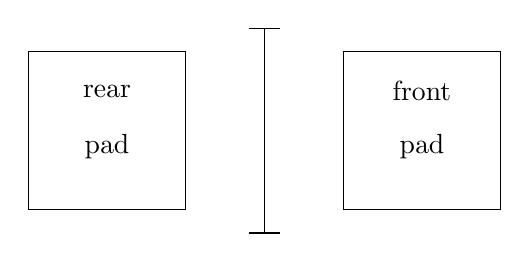
\begin{tikzpicture}
\tikzset{-}
    \draw (-0.2,1.3) -- (0.2,1.3);
\draw (-0.2,-1.3) -- (0.2,-1.3);    
\draw (0,-1.3) -- (0,1.3);
\draw (1,-1) rectangle (3,1);
\path node at (2, 0.5) {front};
\path node at (2, -0.2) {pad};
\draw (-1,-1) rectangle (-3,1);
\path node at (-2, 0.5) {rear};
\path node at (-2, -0.2) {pad};
  \end{tikzpicture}
\end{center}
\item Rules:

\item [] When it moves, it cannot hit people
\item We can use a simple graph to summarize all operations
\item Fig 1.2

\begin{tikzpicture}
\node[state] (closed) {closed};
  \node[state] (open) [right of=closed] {open};

   \path (closed) edge[loop below]  node {rear, both, neither} (closed)
         (closed) edge[bend left, above]              node {front} (open)
         (open) edge[bend left, below]              node {neither} (closed)
         (open) edge[loop right] node {front, rear, both} (open);
\end{tikzpicture}

\item Single bit memory (open and closed)
\item Automaton (single)

\item [] automata (plural)

\end{itemize}\end{frame} \begin{frame}[allowframebreaks] \frametitle{Examples of automata}
  \begin{itemize}
  \item Fig 1.4: a state diagram

  \begin{tikzpicture}
  \node[state,initial] (q_1) {$q_1$};
  \node[state,accepting, right of=q_1] (q_2)  {$q_2$};
  \node[state, right of=q_2] (q_3)  {$q_3$};

  \draw (q_1) edge[loop above]    node {$0$} (q_1)
        (q_1) edge[above]  node {$1$} (q_2)
        (q_2) edge[loop above]    node {$1$} (q_2)
        (q_2) edge[bend left, above] node {$0$} (q_3)
        (q_3) edge[bend left, below] node {$0,1$} (q_2);
\end{tikzpicture}

\item [] states: $q_1, q_2, q_3$

\item [] starting states: $q_1$

\item [] accept state $q_2$ (double circle)
\item Example: running an input string 1101
  \begin{equation*}
    q_1
\rightarrow q_2 \rightarrow
q_2 \rightarrow q_3 
\rightarrow q_2
\end{equation*}
This string is accepted
\item Example: running 10
    \begin{equation*}
    q_1
\rightarrow q_2 \rightarrow
q_2 \rightarrow q_3 
\end{equation*}
$q_3$ is not an accept state, so the string is rejected
\item What are all strings accepted?
\item [] We will say what this set is
\item [] Unfortunately, it may not be always easy to know the set

\end{itemize}\end{frame}


\begin{frame}[allowframebreaks] \frametitle{Formal definition}
We formally define a state diagram as a 5-tuple $(Q,\sigma, \Delta, q_0, F)$
  \begin{itemize}

\item $Q$: set of states. It is a \alert{finite} set
\item $\Sigma$: alphabet (i.e., set of characters in input string). It is a finite set
\item $\delta: Q \times \Sigma \rightarrow Q$: transition function
\item [] This is the most complicated part of the definition. We explain it by an example
  later
\item $q_0 \in Q$: start state
\item $F \subset Q$: set of accept states

\item For the example given above,
\begin{gather*}
  Q=\{q_1,q_2, q_3\}\\
\Sigma=\{0,1\}\\
q_0 = q_1 \\
F=\{q_2\}
\end{gather*}
\item The $\delta$ function:
  \begin{center}
  \begin{tabular}{c|cc}
& 0 & 1\\ \hline
$q_1$ & $q_1$ & $q_2$\\
$q_2$ & $q_3$ & $q_2$\\
$q_3$ & $q_2$ & $q_2$
  \end{tabular}
\end{center}
\item Language of $M$: all strings accepted by $M$. 
Denoted as
\begin{equation*}
A=L(M)
\end{equation*}
\item Figure 1.4:
  \begin{equation*}
    \begin{split}
    A=\{
w \mid & w: \text{ at least one 1, even \# 0} \\
& \text{after the last 1}\}
\end{split}
  \end{equation*}
\end{itemize}
\end{frame}

\begin{frame}[allowframebreaks] \frametitle{Example 1.7}
  \begin{itemize}
  \item Figure 1.8

    \begin{tikzpicture}
\node[state,initial] (q_1) {$q_1$};
\node[state,accepting] (q_2) [right of=q_1] {$q_2$};      

  \path (q_1) edge[bend left, above]  node {$1$} (q_2)
        (q_1) edge[loop above] node {$0$} (q_1)
        (q_2) edge[loop above] node {$1$} (q_2)
        (q_2) edge[bend left, below]  node {$0$} (q_1);
      \end{tikzpicture}
\item $M=(\{q_1,q_2\}, \{0,1\},
\delta, q_1, \{q_2\})$
\item What is $L(M)$ ?
Anything ends with 1

\item How to think about this ?

\item Before the last input character, we must
  be at $q_1$ or $q_2$. Then only if the last is 1 we
  can reach $q_2$ to get accepted
\end{itemize}\end{frame} \begin{frame}[allowframebreaks] \frametitle{Example 1.11}
  \begin{itemize}
  \item Fig 1.12
    \begin{center}
    \begin{tikzpicture}
  \node[state,initial]   (s)                      {$s$};
  \node[state,accepting] (q_1) [below left of=s]  {$q_1$};
  \node[state]           (q_2) [below of=q_1]     {$q_2$};
  \node[state,accepting] (r_1) [below right of=s] {$r_1$};
  \node[state]           (r_2) [below of=r_1]     {$r_2$};

  \path[->]
  (s)   edge [above]             node {a} (q_1)
        edge [above]             node {b} (r_1)
  (q_1) edge [loop left]  node {a} (   )
        edge [bend left,right]  node {b} (q_2)
  (q_2) edge [loop left]  node {b} (   )
        edge [bend left,left]  node {a} (q_1)
  (r_1) edge [loop right] node {b} (   )
        edge [bend left, right]  node {a} (r_2)
  (r_2) edge [loop right] node {a} (   )
        edge [bend left, left]  node {b} (r_1);      
    \end{tikzpicture}
  \end{center}
\item $L(M)=?$
  \begin{equation*}
    a\ldots a, b \ldots b
  \end{equation*}

$\ldots$ can be any string of $a$ and $b$
\end{itemize}\end{frame}



\begin{frame}[allowframebreaks] \frametitle{Example 1.13}
  \begin{itemize}
  \item Figure 1.14

    \begin{tikzpicture}[node distance=4cm]
 \node[state,accepting,initial] (q_0) {$q_0$};
  \node[state] (q_1) [above right of=q_0] {$q_1$};
  \node[state] (q_2) [below right of=q_1] {$q_2$};

  \path 
        (q_1) edge[bend right=15, above]  node [rotate = 45] {$2, \langle  \text{reset}\rangle$} (q_0)
  (q_0) edge[bend right=15, above] node {$1$} (q_1)
        (q_0) edge[loop below]  node {$0, \langle  \text{reset}\rangle$} (q_0)
        (q_1) edge[loop above]  node {$0$} (q_1)
        (q_1) edge[bend left=15, above] node {$1$} (q_2)
        (q_2) edge[bend left=15, above] node {$2$} (q_1)
        (q_2) edge[loop right]   node {$0$} (q_2)
        (q_0) edge[bend left=15, above] node {$2$} (q_2)
        (q_2) edge[bend left=15, below] node {$1, \langle  \text{reset}\rangle$} (q_0);    
      \end{tikzpicture}
\item $\Sigma=
\{\langle  reset\rangle,0,1,2\}$
\begin{gather*}
  L(M)=\ldots \ldots\langle  reset\rangle\ldots\langle  reset\rangle\ldots
\\
 =\{\mbox{sum of the
    last segment } \mod 3 = 0\}
\end{gather*}
\item Example:
  \begin{equation*}
    10\langle  reset\rangle22\langle  reset\rangle012
  \end{equation*}
\item Running this string
  \begin{equation*}
    \begin{split}
      &      q_0 \xrightarrow{1} q_1 \xrightarrow{0} q_1
      \xrightarrow{\langle reset \rangle} q_0 
            \xrightarrow{2} q_2 \xrightarrow{2} q_1 \\
&      \xrightarrow{\langle reset \rangle} q_0
      \xrightarrow{0} q_0 \xrightarrow{1} q_1 \xrightarrow{2} q_0
    \end{split}
  \end{equation*}
Accepted.
\end{itemize}\end{frame} \begin{frame}[allowframebreaks] \frametitle{Formal Definition of Computation}
  \begin{itemize}
\item $M$ accepts $w=w_1 \cdots w_n$ if $\exists$ states

 $r_0 \cdots r_n$ such that
  \begin{enumerate}
  \item $r_0 = q_0$
  \item $\delta(r_i, w_{i+1})= r_{i+1}, i = 0, \ldots, n-1$
  \item $r_n \in F$
  \end{enumerate}
\item \alert{Definition}:
  a language is regular if recognized by some automata
\end{itemize}\end{frame} \begin{frame}[allowframebreaks] \frametitle{Designing Automata}
  \begin{itemize}
\item Given a language, how do we construct a machine to recognize it?
\item Basically we need to get a state diagram (where the number
  of states is finite)
\item An automaton recognizing $\{0,1\}$ strings with odd
\# of 1's 

\item []Fig 1.20

\begin{center}
    \begin{tikzpicture}
\node[state,initial] (q_e) {$q_e$};
\node[state,accepting] (q_o) [right of=q_e] {$q_o$};      

  \path (q_e) edge[bend left, above]  node {$1$} (q_o)
        (q_e) edge[loop above] node {$0$} (q_e)
        (q_o) edge[loop above] node {$0$} (q_o)
        (q_o) edge[bend left, below]  node {$1$} (q_e);
      \end{tikzpicture}
    \end{center}
\item Example

\item [] 01
  \begin{equation*}
    q_e \xrightarrow{0} q_e \xrightarrow{1} q_o
  \end{equation*}
  010101
  \begin{equation*}
    q_e \xrightarrow{0} q_e \xrightarrow{1} q_o
    \xrightarrow{0} q_o \xrightarrow{1} q_e \xrightarrow{0} q_e
    \xrightarrow{1} q_o
  \end{equation*}
  
\item Two ways to think about the design
  \begin{itemize}
  \item After the first 1, we go to $q_o$. Subsequently, every $1, \ldots, 1$ pair is cancelled out by
  \begin{equation*}
q_o \xrightarrow{1} q_e \rightarrow \cdots \rightarrow q_e
    \xrightarrow{1} q_o
  \end{equation*}
\item $q_e, q_o$ respectively remember whether the number of 1's
  so far is even or odd
  \end{itemize}
\item Example 1.21
  
\item [] strings contain 001

\item [] Fig 1.22

\begin{center}
    \begin{tikzpicture}
\node[state,initial] (q) {$q$};
\node[state] (q_0) [right of=q] {$q_0$};
\node[state] (q_00) [right of=q_0] {$q_{00}$};
\node[state,accepting] (q_001) [right of=q_00] {$q_{001}$};      
  \path 
        (q) edge[loop above] node {$1$} (q)
  (q) edge[bend left, above]  node {$0$} (q_0)
  (q_0) edge[bend left, below]  node {$1$} (q)
  (q_0) edge[above]  node {$0$} (q_00)
  (q_00) edge[loop above] node {$0$} (q_00)
  (q_00) edge[above]  node {$1$} (q_001)  
   (q_001) edge[loop below] node {$0,1$} (q_001);
      \end{tikzpicture}
    \end{center}
  \item $q_0, q_{00}$ indicate that before the current input character,
    we have 0 and 00, respectively
\end{itemize}\end{frame} \begin{frame}[allowframebreaks] \frametitle{Regular Operations}
  \begin{itemize}
\item Regular operations can be used to study whether languages are regular or not

\item  That is, we aim to check if for a given language,
  where there are finite automata to recognize it or not
\item Three definitions

\item [] $A,B$ are given languages
\begin{itemize}
\item union
  \begin{equation*}
  A \cup B
\end{equation*}
\item concatenation
  \begin{equation*}
  A\circ B=\{xy\mid x\in A, y \in B\}
\end{equation*}
\item star:
  \begin{equation*}
  A^*=\{x_1 \cdots x_k\mid
k \geq 0, x_i \in A\}
\end{equation*}
\end{itemize}
\item If $k=0$, what do we mean
  \begin{equation*}
    x_1 \cdots x_k?
  \end{equation*}
  We define
  \begin{equation*}
     \epsilon: \text{ empty string}
   \end{equation*}
in this situation
\item Thus
  \begin{equation*}
   \epsilon \in A^*
 \end{equation*}
\item Example
  \begin{equation*}
    \begin{split}
& \Sigma =\{a, \ldots, z\}\\
& A=\{good, bad\} \\
& B=\{boy,girl\} \\
& A\circ B=
\{goodboy, \ldots \}\\
& A^*: \{\epsilon, good, bad, goodgood, \ldots\}
\end{split}
\end{equation*}
\item We say an operation $R$ is \alert{closed} if the
  following property holds
  \begin{center}
if $x\in A, y \in A$, then $xRy \in A$
\end{center}
Example: $N=\{1,2,\ldots\}$ is closed under multiplication
\item Th 1.25: regular languages are closed under the union operation

  \begin{equation*}
    \begin{split}
&    A_1, A_2 \text{ are regular languages} \\
\Rightarrow & A_1 \cup A_2 \text{is regular}
  \end{split}
\end{equation*}

\item Proof
\item [] Assume we are given two automata
  \begin{eqnarray*}
&& M_1 =(Q_1, \Sigma, \delta_1, q_1, F_1)\\
&& M_2 =(Q_2, \Sigma, \delta_2, q_2, F_2)\\
  \end{eqnarray*}
\item Construct a new machine
  \begin{eqnarray*}
&& M =(Q, \Sigma, \delta, q, F)\\
&& Q=\{(r_1,r_2)\mid r_1 \in Q_1, r_2 \in Q_2\}\\
&& \delta((r_1,r_2),a)=(\delta_1(r_1,a), \delta_2(r_2,a))\\
&& q_0 = (q_1,q_2)\\
&& F=\{(r_1, r_2) \mid r_1 \in F_1 
\text{ or } r_2 \in F_2\}
  \end{eqnarray*}
\item Example: combining
  \begin{equation*}
    \begin{split}
      & \{ w \mid w \text{ has an odd \# 1's} \} \cup \\
      & \{ w \mid w \text{ has an odd \# 0's} \}
\end{split}
\end{equation*}
\begin{center}

    \begin{tikzpicture}
\node[state,initial] (q_e) {$q_e$};
\node[state,accepting] (q_o) [right of=q_e] {$q_o$};      

  \path (q_e) edge[bend left, above]  node {$1$} (q_o)
        (q_e) edge[loop above] node {$0$} (q_e)
        (q_o) edge[loop above] node {$0$} (q_o)
        (q_o) edge[bend left, below]  node {$1$} (q_e);
      \end{tikzpicture}

    \begin{tikzpicture}
\node[state,initial] (s_e) {$s_e$};
\node[state,accepting] (s_o) [right of=s_e] {$s_o$};      

  \path (s_e) edge[bend left, above]  node {$0$} (s_o)
        (s_e) edge[loop above] node {$1$} (s_e)
        (s_o) edge[loop above] node {$1$} (s_o)
        (s_o) edge[bend left, below]  node {$0$} (s_e);
      \end{tikzpicture}
    \end{center}
    \begin{center}
    \begin{tikzpicture}
      \node[state,initial] (qese) {$q_e,s_e$};
      \node[state] (qeso) [accepting, above right of = qese] {$q_e,s_o$};
      \node[state] (qose) [accepting, below right of = qese] {$q_o,s_e$};
\node[state,accepting] (qoso) [below right of = qeso] {$q_o,s_o$};                  
\path (qese) edge[bend left, above]  node {$0$} (qeso)
(qeso) edge[bend left, above]  node {$0$} (qese)
(qeso) edge[bend left, above]  node {$1$} (qoso)
(qoso) edge[bend left, above]  node {$1$} (qeso)
(qese) edge[bend left, above]  node {$1$} (qose)
(qose) edge[bend left, above]  node {$1$} (qese)
(qose) edge[bend left, above]  node {$0$} (qoso)
(qoso) edge[bend left, above]  node {$0$} (qose);
      \end{tikzpicture}
    \end{center}
  
\item Is this proof rigourously enough ?
\item [] A formal proof should be done by induction. But we don't
  provide it here
\item Th 1.26: closed under concatenation
  \begin{center}
    If $A, B$ are regular, then $A \circ B$ is regular
  \end{center}
\item [] But the proof is not easy
\item [] It's unclear where to break the input 

\item To easily do the proof,
  we introduce a new technique called \alert{nondeterminism}
  \end{itemize}\end{frame}

\end{document}
